\chapter{Introduction}

Cloud computing became a reality over the last years, and many companies are now moving their data-centers to the cloud. 
A concept that is often linked with cloud computing is Infrastructure as a Service (IaaS): the computational infrastructure of a company can now be seen as a monthly cost instead of a number of different factors. 
Recently, a number of organizations started to replace their relational databases with hybrid solutions (NoSQL DBs, Search Engines, ORDBs). 

These changes are motivated by (\textit{i}) performance improvements on the overall performance of the applications and (\textit{ii}) inability to a RDBMS to provide the same performance of a hybrid solution given a fixed monthly infrastructure cost.

However, not always the companies can exactly measure beforehand the future impact on the performance of their services by making this sort of technological changes (replace RDBMS by another solution).

In a production environment, it is necessary to assure that a database transition will actually bring benefits to the overall performance of the application. To avoid external threats and unknown risks, a database transition must be made in a pragmatic manner on each step of the transition: from the initial hypothesis' to the deployment of the new architecture.


\section{Problem}

The decision to migrate (part of) an application from RDBMSs to NoSQL alternatives, such as Search Engines or Graph Databases, make sense when the alternatives have better performance than the classic RDBMSs and the cost to have a similar performance is significantly higher. 

Several steps are needed in the process of replacing a relational database by a NoSQL alternative. An initial step on transitioning processes could be (\textit{i}) to map the relational schema into the new kind of document. Some works, such as \cite{lombardo2012issues} \cite{zhu2012data} address this sort of problem. Schema mappings across different technologies are, however, very particular to every case. \cite{bahl2014mysql} shows, for example, how a MySQL schema may be represented on MongoDB and Neo4j, both NoSQL DBs.

Another possible initial step on transitioning database technologies could be (\textit{ii}) to prove that the current database infrastructure is breaking some of the requirements of an application, such as the speed of an operation. 

The ``prove'' that the current DB infrastructure is breaking the requirements could be the result of a DB Benchmark or the execution of an automated test, for example. Several Benckmarking Frameworks, such as TPC-H \cite{council2008tpc}, can be used on this step. Automated tests can make use of testing libraries/frameworks, as jUnit \cite{massol2003junit} and rspec \cite{chelimsky2010rspec} or can be implemented from scratch using popular programming languages, as Java and Python.

Database transitioning processes are generally non-standardized and may differ significantly, as revealed on \cite{fabioMartinSM}.  

In this work we assess how Service Level Agreements (SLAs) can be used to help the migrations from RDBMSs to NoSQL solutions and propose a set of Guidelines based on SLAs to justify and assess the transitions from RDBMs to NoSQL alternatives.

\section{Proposed solution}

In this work we propose a set of steps to guide the transition from relational databases to NoSQL ones. The suggested guidelines makes use of Service Level Agreements (SLAs) to guide the whole process. These guidelines are represented on Figure~\ref{fig:guidelinesNoSQL}


\begin{figure}[ht!]
\centering
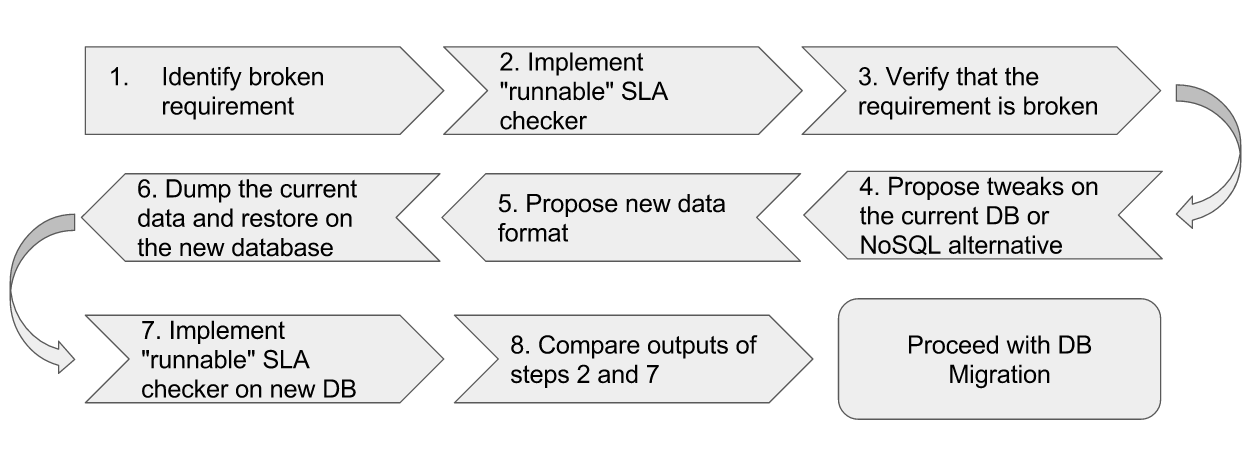
\includegraphics[width=130mm]{guidelines.png}
\caption{Relational to NoSQL Steps.\label{fig:guidelinesNoSQL}}
\end{figure}

The guidelines consist on a total of 9 steps, as follows:


\begin{itemize}
   \item{\textbf{Identify broken requirement} - A database migration is generally motivated by performance issues. The first step of the guidelines is to identify what are the operations that are motivating the database transition. This can an existing requirement or a new one. i.e: In the context of a retail business intelligence application, a possible requirement could be \textit{``I want to have a word cloud from the Twitter Bio from the customers that bought product X, Y or Z. I'd like to wait up to 5 seconds to see this word cloud.''.}}
   \item{\textbf{Implement ``runnable'' SLA checker} - On this step a ``runnable SLA'' is implemented to assure that the current DB infrastructure does not support the requirement. }
   \item{\textbf{Verify that the requirement is broken} - After having the ``runnable SLA'' implemented, it is possible to check that the requirement is not being fulfilled by the current DB infrastructure.}
   \item{\textbf{Propose tweaks on the current DB or NoSQL alternative} - Not always is necessary to change all database infrastructure to address a small problem. SQL tunning, denormalizing tables and creating indexes are popular ways to improve the performance of RDBMSs. In some cases, however, a NoSQL strategy is recommended to avoid extra costs on the ``scale-up'' strategy.}
   \item{\textbf{Propose new data format} - After choosing the new NoSQL database, it is necessary to map the table elements and relations into the new concepts of the chosen NoSQL technology.}
   \item{\textbf{Dump the current data and restore on the new database} - To compare the performance of RDBMS vs NoSQL on a specific scenario, the same amount of data must be present on both DBs. So, a Dump \& Restore procedure is needed on the side of the NoSQL DBs.}
   \item{\textbf{Implement ``runnable'' SLA checker on new DB} - Once the new DB is populated with production data, a new ``runnable'' SLA is needed to compare the results of the proposed architecture and the old architecture}
   \item{\textbf{Compare outputs of steps 2 and 7} - If the new DB architecture fills the gaps of the broken requirements \textit{ and other requirements are not broken with the new architecture}, the DB transition should be made.}
   \item{\textbf{Proceed with DB migration} - On this step, the source code of the application should be updated to match the new Database Architecture. }
\end{itemize}

% % Casos a serem considerados em trabalhos futuros: 
% % > Load Tests
% % > Mapear todos os requisitos / operações da aplicação na nova arquitetura.


% Esqueleto do framework/guidelines

% 1 - Criacao de SLA para cada operacao disponibilizada pelo component: Nesse passo definimos um SLA que tal servico deve obedecer (chamadas a tal endpoint devem retornar em <2s, por ex. Esse SLA servira para ``provar'' que a minha tecnologia + infraestrutura atual nao me atende satisfatoriamente.
% 2 - Criacao de um SLA (suite de testes automatizados ou qualquer coisa definida no SLA@SOI) que mostre que a aplicacao nao respeita o SLA acordado no passo anterior.
% 3 - Proposicao de nova infraestrutura/tecnologia
% 4 - Implementacao e Simulacao
% 6 - Comparacao dos testes antigos e novos
% 7 - Validacao da melhoria e cumprimento do SLA acordado na etapa 01.
% 8 - Monitoramento continuo das operacoes apos a migracao (SLA ativo)

% - A validacao do framework e da app a partir de aplicacoes de exemplo;
% - Open-source app que escuta todas as requisicoes a um servidor (JS-based e server based) e analisa se um SLA foi respeitado apos alguma mudanca;
% - Implementacao com alguma coisa de Open Stack;

\section{Contribution}

In this work, the main contributions are: 

\begin{itemize}
   \item{Proposition of a set of Guidelines based on SLAs to justify and constantly assess the transitions from RDBMs to NoSQL DBs;}
   \item{A Batch PDF-Tokens matcher, available on \cite{pythonBatchPDFTokenMatcher} ;}
   \item{A Systematic mapping study on ``Using SLA to guide database transition to NoSQL on the cloud'', available on \cite{fabioMartinSM};}
   \item{Scenarios that compare the performance of RDBMs with NoSQL alternatives in specific tasks.}
\end{itemize}

\subsection{Publications}

As a result of this work, the following papers were published:

\textit{LEAL, F.; MUSICANTE, M. Todo: Update this reference - using sla to guide database transition to nosql on the cloud: a systematic mapping study.}


\section{Structure of this work}
On this section we presented an overview of this work, giving a brief introduction about the related concepts. The problem and solution that this work aims to solve were also presented on the sections from this chapter. 

On Chapter~\ref{bibreviewChap} we present a detailed view on each concepts that surround this work and explain how each of these concepts are linked with our work. 

On Chapter~\ref{theProblemChap} we extensively detail our problem and the proposed solution.

On Chapter~\ref{validationChap} we present how the guidelines defined on Chapter~\ref{theProblemChap} might be used on a RDBMS to NoSQL transition. 

On Chapter~\ref{conclusionsChap} we present the next steps that are possible from this work. The References that we used on our work are made available after this chapter.  